\section{Preliminary Simulations}
	In order to test if RegCM5 is working on the laboratory's workstation,
		a preliminary simulation was conducted.
	The domain of the simulation is Luzon, centered on Manila, as shown in Figure \ref{fig:proposal-domain}.
	The domain has an area of $\num{130}$ by $\num{124}$ grid cells, with a $\qty{3}{km}$ resolution.
	Data for initial and boundary condition were dated from March to September 1990,
		and the simulation itself is from March to May 1990.
	The run used 24 cores and took 14 hours to complete.
		
	\begin{figure}
		\centering
		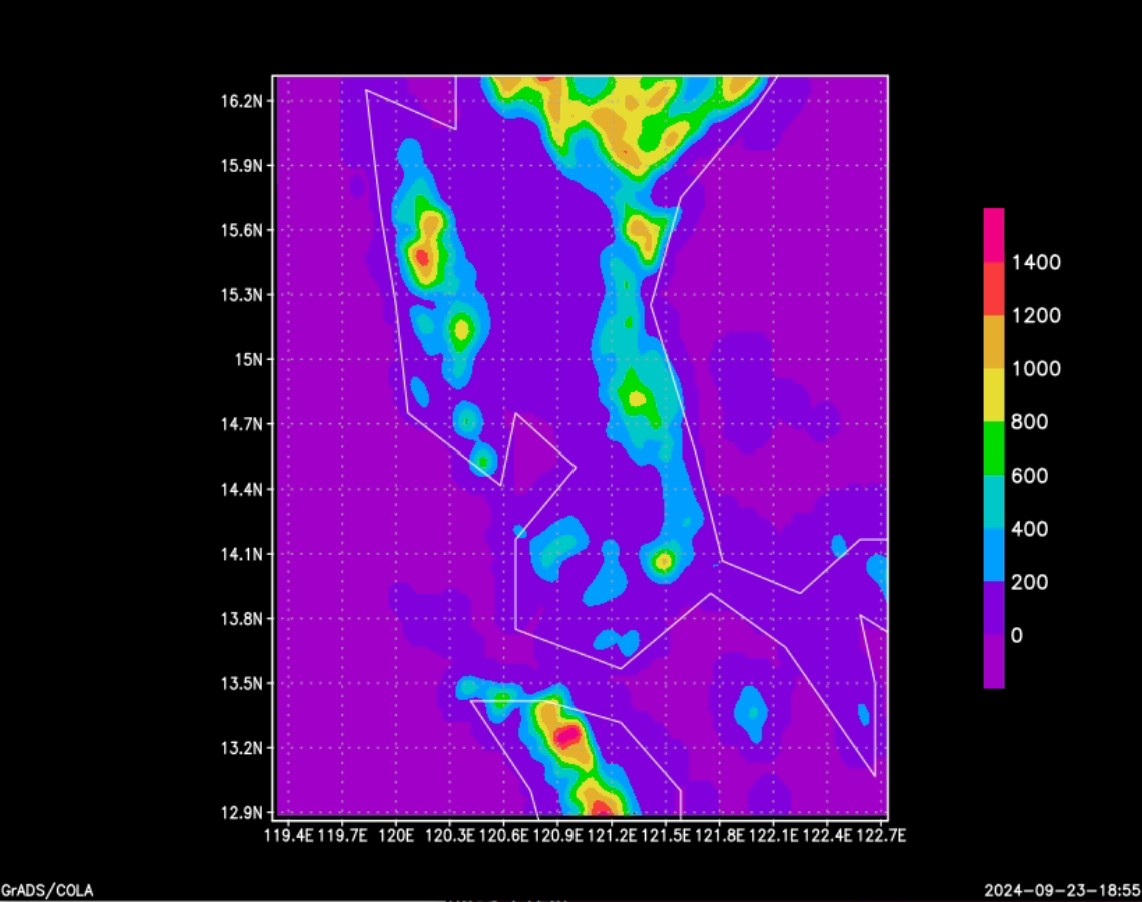
\includegraphics{proposal-domain}
		\caption{
			Surface model elevation of the domain used in the preliminary simulation.
			Domain is centered on Manila (\ang{14;35} N, \ang{121} E),
				with a grid of $\num{130}$ by $\num{124}$ cells
				and a resolution of $\qty{3}{km}$.
			Units of the elevation are in meters.
		}
		\label{fig:proposal-domain}
	\end{figure}
	
	\begin{figure}
		\centering
		\begin{subfigure}{\textwidth}
			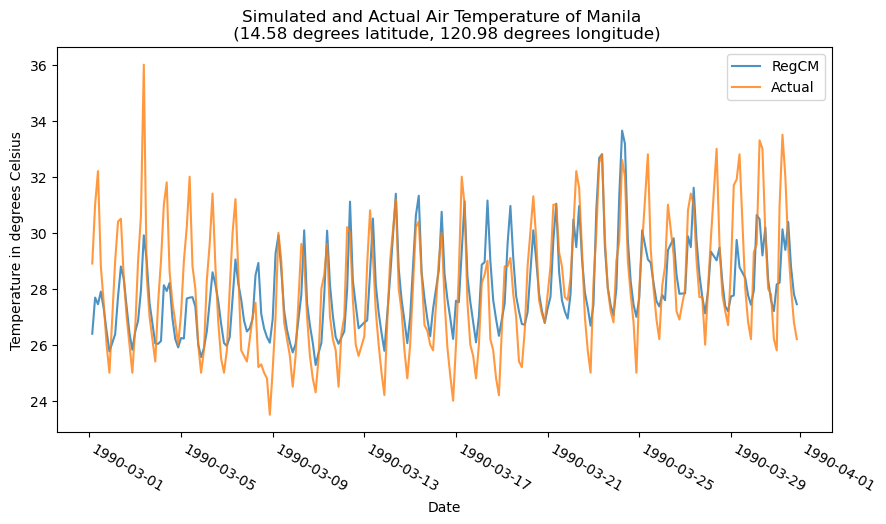
\includegraphics[width=\textwidth]{proposal-manila-both}
		\end{subfigure}
		\begin{subfigure}{\textwidth}
			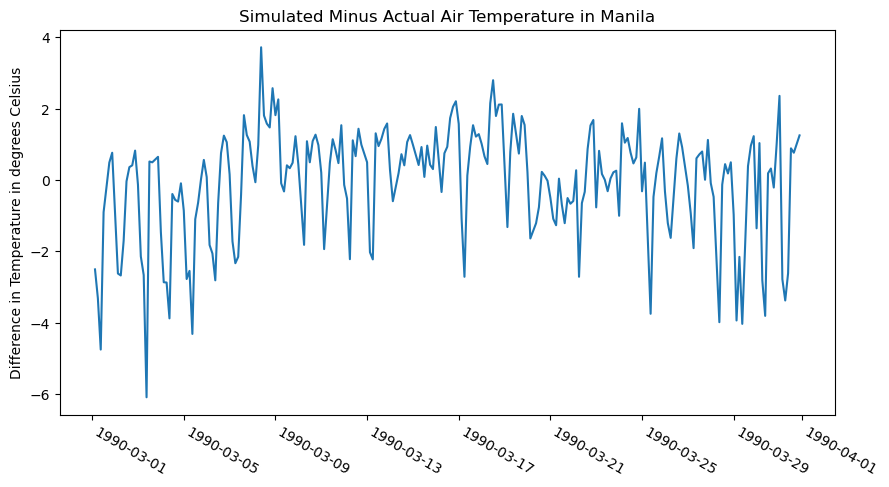
\includegraphics[width=\textwidth]{proposal-manila-difference}
		\end{subfigure}
		\caption{
			Graphs of the simulated and actual near-surface air temperature of Manila (\ang{14.58} N, \ang{120.98} E).
		}
		\label{fig:sdlfjdlf}
	\end{figure}
	
	

\section{Budget and Timeline}